%%%%%%%%%%%%%%%%%%%% author.tex %%%%%%%%%%%%%%%%%%%%%%%%%%%%%%%%%%%
%
% sample root file for your "contribution" to a contributed volume
%
% Use this file as a template for your own input.
%
%%%%%%%%%%%%%%%% Springer %%%%%%%%%%%%%%%%%%%%%%%%%%%%%%%%%%%%%%%%%


%% RECOMMENDED %%%%%%%%%%%%%%%%%%%%%%%%%%%%%%%%%%%%%%%%%%%%%%%%%%%
%\documentclass[graybox]{svmult}
%
%% choose options for [] as required from the list
%% in the Reference Guide
%
%\usepackage{mathptmx}       % selects Times Roman as basic font
%\usepackage{helvet}         % selects Helvetica as sans-serif font
%\usepackage{courier}        % selects Courier as typewriter font
%\usepackage{type1cm}        % activate if the above 3 fonts are
                             % not available on your system
%
%\usepackage{makeidx}         % allows index generation
%\usepackage{graphicx}        % standard LaTeX graphics tool
%                             % when including figure files
%\usepackage{multicol}        % used for the two-column index
%\usepackage[bottom]{footmisc}% places footnotes at page bottom
%
%% see the list of further useful packages
%% in the Reference Guide
%
%\makeindex             % used for the subject index
%                       % please use the style svind.ist with
%                       % your makeindex program
%
%%%%%%%%%%%%%%%%%%%%%%%%%%%%%%%%%%%%%%%%%%%%%%%%%%%%%%%%%%%%%%%%%%%%%%%%%%%%%%%%%%%%%%%%%%
%
%\begin{document}

\title{Buildings}
% Use \titlerunning{Short Title} for an abbreviated version of
% your contribution title if the original one is too long
\author{
    \textbf{Adam Zsarnóczay}
    \and Jack W. Baker}
\tocauthor{}
\authorrunning{Zsarnóczay and Baker}
% Use \authorrunning{Short Title} for an abbreviated version of
% your contribution title if the original one is too long
%\institute{Name of First Author \at Name, Address of Institute, %\email{name@email.address}
%\and Name of Second Author \at Name, Address of Institute %\email{name@email.address}}
%
% Use the package "url.sty" to avoid
% problems with special characters
% used in your e-mail or web address
%
\maketitle

Buildings are arguably the most important asset type when it comes to direct consequences of a natural disaster. A severely damaged or collapsed building may result in loss of life, injuries, and significant capital losses. Seismic performance assessment of buildings has received a lot of attention from the research community and funding agencies in the past few decades (\cite{atc1985atc13, fema1997guidelines, fajfar2004performancebased}; and \cite{kircher2006hazus}). Consequently, the most sophisticated and mature methods are available in that area \citep{atc2012p-58}. Several researchers have focused on adopting these methods for other asset types \citep{werner2006redars, chmielewski2016response} and for other types of hazards (\cite{vickery2006hazus, bernardini2015performance, attary2017performancebased, barbato2013performancebased}; and \cite{lange2014application}). Although this has led to similar methods being used for various types of assets, some of the synergies between these methods remain un-utilized in research.

Historically, two different approaches have been developed for performance assessment of buildings. Until recently, the methods and models used in these approaches improved in parallel (Figure \ref{fig:perf_PBEapproaches}):

\begin{itemize}
    \item Large-scale simulations of distributed building inventories required idealized, efficient models that provided sufficiently accurate performance estimates while limiting the computational workload to make the simulations feasible. The most popular example of such an approach is the HAZUS framework that has been developed for earthquake \citep{fema2018earthquaketechnical}, hurricane \citep{fema2018hurricaneuser}, and tsunami hazards \citep{fema2017tsunamitechnical}. HAZUS and similar methods typically take path I or II in Figure \ref{fig:perf_PBEapproaches} and estimate the consequences of a disaster using vulnerability or fragility functions that link the intensity of the natural hazard directly to measures of damage and losses at the building level; and
    \item The assessment of individual buildings has been moving from a holistic towards a component-based approach. Instead of trying to characterize the building damage as a whole, recent performance-based engineering (PBE) methods disaggregate buildings into sets of components and apply separate models (i.e., functions) to estimate the damage and losses for each component. These methods require a detailed description of the building and its behavior under the natural hazard event, necessitating the simulation of building response following path III in Figure \ref{fig:perf_PBEapproaches}. In return, they provide high-resolution information about the damage and losses that allow better understanding of the building's performance. FEMA P-58 \citep{atc2018p-58-1} represents the state-of-the-art in high-fidelity seismic performance assessment for buildings. Researchers have recently been developing similar PBE methodologies for other hazards (e.g. \cite{barbato2013performancebased, ouyang2020performance}; and  \cite{attary2017performancebased}).
\end{itemize}

The two approaches presented above were traditionally separated because neither the computational resources nor the detailed description of assets were available to apply the high-fidelity models and methods at a large, regional scale. Recent advances in computational resources, data harvesting, and processing (see Part \ref{part:cross}) are now bridging the gap between these methods, suggesting that integrated multi-fidelity performance assessment of large asset portfolios will become available for researchers in the near future \citep{deierlein2020cloud}.

\begin{figure}[htb]
    \centering
    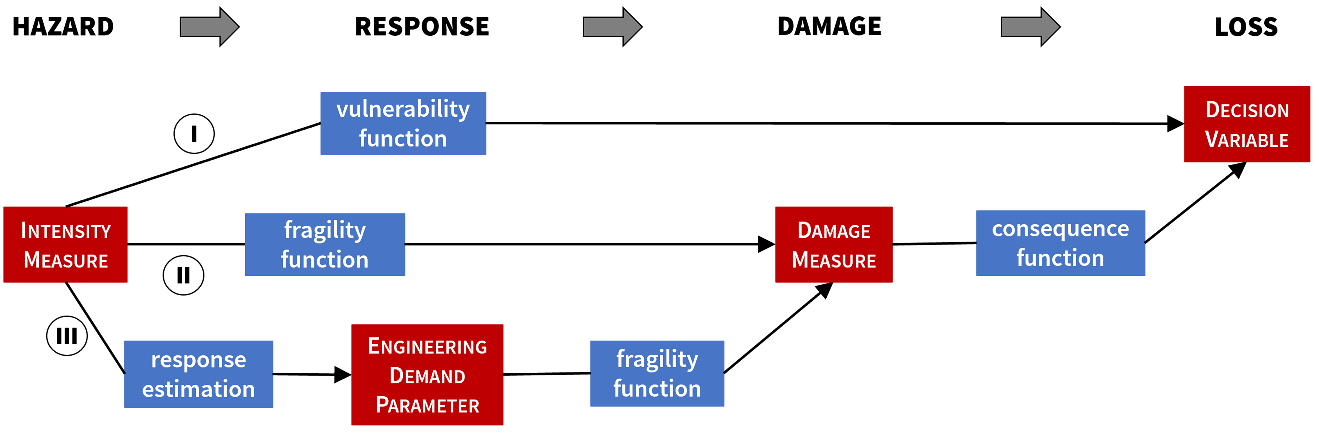
\includegraphics[width=0.9\textwidth, angle = 0]{Figures/PBEapproaches.pdf}
    \caption{Schematic workflows for asset performance assessment \citep{deierlein2020cloud}.}
    \label{fig:perf_PBEapproaches}
\end{figure}
 
\section{Input and Output Data}
\label{sec:perf_bldg_io}

\subsection{Input Data}

The following types of data are required to evaluate the performance of a building:

\paragraph{Hazard characterization} When the building performance is not conditioned on a particular disaster scenario but is evaluated considering all possible scenarios within a time period, the likelihood of each possible scenario needs to be estimated (e.g., time-based assessment in FEMA P-58 \cite{atc2018p-58-1}). The hazard curve describes the rate of exceeding various levels of an intensity measure (IM) over the time period of interest. More information about the description of the hazard is provided in Chapter \ref{chapter:haz_shaking}.

\paragraph{Intensity Measures} Efficient building performance assessment methods directly link IMs to damage measures and decision variables using fragility functions and vulnerability functions, respectively. For such methods, the inputs need to characterize the intensity of the event either through parameters of a distribution function (e.g., mean, standard deviation) or by directly providing samples of the IMs. More information about obtaining IM data is available in Chapter \ref{chapter:haz_shaking}.

\paragraph{Engineering Demand Parameters (EDPs)} High-fidelity building performance assessment uses EDPs as proxies for the detailed history of building response under a natural disaster event. Such EDPs should have high correlation with the building damage of interest and should be estimable with sufficiently high accuracy through numerical analysis. Estimation of EDPs first requires a building response model that is typically created in one of the environments listed in Chapter \ref{chapter:res_struct}. Second, the building model needs to be excited with loads that correspond to a particular hazard event. The inputs required for these models and analysis have been described in previous parts of this report.

Engineering demand parameters are extracted from the structural response simulation. Seismic performance assessment often uses peak responses at every story such as peak story drift ratios and peak floor accelerations \citep{atc2018p-58-1}. Other hazards result in different response histories and damage, and they are characterized by other EDPs, such as external pressures \citep{ouyang2020performance} or maximum inundation depth \citep{reese2011empirical}. 

\paragraph{Component characteristics} Depending on the complexity of the performance assessment method and data availability, buildings are described as a system of components or component-groups. For example, the component-group-based approach followed by HAZUS \citep{fema2011earthquaketechnical} aggregates structural components, non-structural components, and contents into three groups. The FEMA P58 method represents the other end of the spectrum; it disaggregates the building into units of components with identical behavior. The component-group-based method typically requires fewer and more generic inputs such as the type of structural system and the occupancy type to infer component behavior. The more detailed methods use the quantity, direction, and location of each component unit on each floor of the building to estimate their damage.

\paragraph{Fragility functions} Fragility functions describe the likelihood of exceeding a particular damage state as a function of IM or EDP magnitude, (see Figure \ref{fig:perf_PBEapproaches} and \citep{baker2021seismic}). Many fragility functions are publicly available, and there is open discussion about their improvement for the seismic performance estimation of buildings (e.g. \cite{silva2019current}). FEMA P-58 enables sophisticated analysis for seismic hazards by providing \citep{atc2012p-58} and continually revising \citep{atc2018p-58-1} a database with detailed description of more than 700 types of components. The HAZUS platform includes fragility and vulnerability functions for component-groups for various hazards, but the development of publicly-available functions that would allow more detailed assessment under wind and water hazards is a topic of active research.

\paragraph{Vulnerability and consequence functions} Vulnerability and consequence functions describe losses from a disaster as a function of its intensity and the experienced structural damage, respectively. Vulnerability functions are more efficient because they do not require information about the damage incurred, but their estimates have more uncertainty. Vulnerability functions typically describe the consequences at a building-level (e.g., HAZUS), while consequence functions can use more detailed information (e.g., FEMA P-58) about the damage. Each damage state has its corresponding set of consequence functions. These functions are defined by additional input data such as repair cost per component unit, affected area for calculation of injuries, or the expected downtime until the building can be used by its occupants. The description and propagation of uncertainty in these functions is an important part of the calculation method. Consequences that are primarily a function of damage within the building and not affected by the performance of other parts of the civil infrastructure are often referred to as direct consequences. Vulnerability and consequence functions can estimate such outcomes well.

\subsection{Output Data}

\noindent One or more of the following outputs are produced to describe building performance:

\paragraph{Damage Measures (DMs)} Damage in buildings is quantified through damage measures that identify the Damage State (DS) of the investigated building or component. Component damages are classified into a finite number of damage states, so that each DS groups damage scenarios with similar consequences together. Performance assessment is typically executed in a stochastic framework; the DMs are considered random, and the raw results of the assessment are at least thousands of samples of each output variable. Therefore, interpretation and visualization of the results is an important part of the process. The majority of applications focus on mean or median values to describe central tendencies, with the 10th and 90th percentiles used to illustrate the variability of results. High-performance computing and the improvement in the quality of input data create the incentive to improve estimates of the tails of the distributions and to look at the joint distribution of the variables. These analyses reveal details of complex systems that are might be overlooked when focusing only at central tendencies.

\paragraph{Decision variables (DVs)} Decision variables describe the losses due to the natural hazard and are used to characterize the performance of the building and meant to eventually drive decision- and policy-making. Each type of loss has its own DV, such as number of injuries, repair cost, business interruption time, etc.

\paragraph{Indirect consequences} The influence of building damage on surrounding buildings and infrastructure is challenging to model because of the scarcity of data that could be used for calibration; the substantial increase in the complexity of the analysis when dependencies between buildings needs to be considered. Decision variables in this group include non-immediate injuries and hospital demand, displaced households and short-term shelter needs, business interruption costs, demand surge, and its influence on reconstruction cost and downtime estimates. Modeling and simulation of these  outcomes is discussed in Part \ref{part:recovery} of this report.

\section{Modeling Approaches}
\label{sec:perf_bldg_methods}

The main assumption of the widely used stochastic model for building performance assessment is that the uncertainty in the DVs can be estimated through a series of independent calculations. This approach has been developed in the Pacific Earthquake Engineering Research Center (PEER); it is often referred to as the PEER performance assessment framework or simply the PEER ``triple integral'' (see Figure \ref{fig:intro_PBE_framework}, \cite{moehle2004framework}, and \cite{porter2001assemblybased}):

\begin{enumerate}
    \item Describe a set of IM levels (e.g., spectral acceleration intensities) and corresponding likelihoods based on the hazard at the building location over a given time period;
    \item Describe the building response through EDPs at each IM level;
    \item Describe component or component-group DSs given the simulated EDP distributions;
    \item Describe consequences using DVs given the estimated DS of each component or component-group; and
    \item Aggregate DVs from all components or component-groups in the building.
\end{enumerate}

Depending on which path is taken from Figure \ref{fig:perf_PBEapproaches}, one or more of the steps above can be merged. If calculations are performed independently, the models used for these calculations are decoupled (e.g., the DS for two different IM levels is assumed identical if the IMs generate identical EDPs). These steps are the basis of the widely used HAZUS models, and they were the foundation of the FEMA P58 method that is currently considered the state-of-the-art for seismic performance assessment of buildings.

Although sophisticated performance assessment methods promise more information about building performance, their veracity demands more detailed input data about the building and its components. Consideration of the uncertainty that stems from the limited amount of building information available is essential for a robust performance evaluation \citep{bradley2013critical}. The methods available for quantification and propagation of such uncertainty are discussed in Chapter \ref{chapter:uq}.

Under non-seismic hazards, there is no equivalent of the FEMA P58 method that would enable high-fidelity building performance assessment. This partly stems from the lack of publicly available high-quality databases---which would drive more sophisticated model development---and from the different nature of the problem. The impact and disruption of earthquakes and hurricanes are very different in both spatial and temporal distribution, with hurricanes having a severe impact on a larger region over a longer time period. Therefore, the focus for hurricane and flood models have always tended to be more regional and capturing the detailed response of individual structures receives less attention. 

\section{Research Gaps and Needs}
\label{sec:perf_bldg_gaps}

The integration of multiple hazards and multiple asset types in a simulation framework is an essential step towards a comprehensive performance assessment for the built environment. It is important to recognize the difference between multiple hazard studies and multi-hazard studies. Following the naming convention suggested by \citet{bruneau2017state}, the former studies consider multiple, independent hazards in an area, while the latter studies consider the interactions and cascading effects among those hazards as well. In a multi-hazard analysis, the majority of the resulting risk is not from concurrent extreme events because the probability of two of such events happening simultaneously is very low. The characterization and modeling of more frequent hazards becomes more important and influential to the results. There are already several examples of multi-hazard studies in the literature for a wide range of hazard and asset types: earthquake mainshock and aftershock (e.g., \cite{nazari2015effect, zhang2013damage}); ground shaking, liquefaction, and landslides (e.g., \cite{elgamal2008three, kojima2014large}); earthquake and tsunami (e.g., \cite{akiyama2014reliability, carey2019multihazard}); hurricane wind, windborne debris, storm surge (e.g., \cite{lin2010windborne, park2014abv}) and rainwater (e.g., \cite{pita2012assessment}); and flood and sea level rise (e.g., \cite{hinkel2014coastal}). It would also be important to model interactions not only at the hazard level (e.g., \cite{gill2014reviewing}, but also include site effects, disruptions of systems, and system-level social and economic consequences. Analyses that model interactions beyond the hazard level are referred to as Level II interactions by \citet{zaghi2016establishing}.

Consideration of the time-dependency of the hazard (e.g., non-Poissonian earthquake models, and the effect of climate change on wind and water hazards), the structural response and performance (e.g., the effect of aging, retrofitting, and maintenance in general) are gaps in the widely used frameworks that researchers are working to fill (e.g., \cite{gavrilovic2020multi, choe2008probabilistic}; and \cite{pitilakis2014consideration}). Note: bridges have traditionally received more attention than buildings.

The consideration of non-structural components has improved substantially for seismic hazards, but disaggregating their contribution from the structural ones would also enhance the performance assessment under other hazards and in a multi-hazard setting. Besides better characterizing of losses due to non-structural damage, modeling the contribution of these building components to the strength and stiffness of buildings is also an important component of more realistic simulations (e.g., \cite{filiatrault2014performance, welch2016nonstructural})

Constructing a performance model for high-fidelity analyses is also a significant challenge that has only been tackled by proprietary software such as \citeprgm{SP3}. There is no publicly available rule set that could be used to populate a large inventory of buildings with the types, locations, and quantities of components based on the limited amount of building information available for regional-scale assessments. A similar, but distinct problem is the automated model definition for response estimation. That task has received more attention in recent years (e.g., \cite{guan2020python, xiong2016nonlinear}) as well as methods that can produce high-fidelity results without the need to explicitly model and simulate building response (e.g., \cite{zou2020surrogate}).

Epistemic uncertainties (i.e., model-to-model variability) and the bias introduced by idealized models in performance assessment should be taken into consideration (e.g., \cite{aslani2005probability, schotanus2004seismic}) as well as the influence of correlations between EDPs \citep{shome2009comparison} and damage and loss models within a building \citep{ramirez2009building}.

Many of the existing models and methods for performance assessment have not been validated, and new models are rarely compared to existing ones in the literature. Different approaches to model development lead to different results. Even if an identical building class is considered, there can be large variation in the predictions of these. For example, \citet{crowley2014epistemic} shows 60\% coefficient of variation in collapse probability among 24 different models for European reinforced concrete moment frames. This practice risks introducing bias in the performance assessment results and reduces the credibility of the methods. \citet{silva2019current} provides a set of recommendations to improve the reliability of these models.

\section{Software and Systems}
\label{sec:perf_bldg_tools}

The following is a list of software that provides features required for state-of-the-art research in building performance assessment:
% \newline

\paragraph{CAPRA} Development of the Comprehensive Approach to Probabilistic Risk Assessment (\citeprgm{CAPRA}) platform was initially supported by the World Bank and the Inter-American Development Bank; it has been managed by Uniandes (Universidad de los Andes in Colombia) since 2017. CAPRA is designed to become a multi-hazard framework based on several modules that handle different tasks of the risk assessment workflow. The currently available modules allow risk assessment using vulnerability functions for several types of hazards (e.g., earthquake, hurricane, and flood). The open source CAPRA framework uses Visual Basic.NET and provides applications in a Windows environment.

\paragraph{MAEViz} 
Developed by the Mid-America Earthquake Center (MAE), \citeprgm{MAEViz} is based on the HAZUS methodology for scenario risk assessment that allows users to write their own extensions. Through these added modules, its functionality is not limited to building performance assessment and allows analysis of infrastructure and lifeline performance as well as indirect consequences in the region. It uses a Windows-based application with a user interface to guide the user through the analysis. MAEViz is open source and has been integrated into several platforms in the U.S. [e.g., ERGO, mHARP] and in Europe [e.g., SYNER-G \citep{pitilakis2014synerg} and HAZturk \citep{karaman2008earthquake}].

\paragraph{HAZUS 4.2} The FEMA-supported \citeprgm{HAZUS4x2} tool was already introduced in Chapter \ref{chapter:haz_shaking}. The damage and loss assessment modules in the HAZUS earthquake methodology use a component-group-based approach and categorize components into structural, non-structural, and content groups. HAZUS methods for other hazards do not separate structural and non-structural components. They provide building-level estimates of decision variables. Decision variables cover a wide range of direct and indirect consequences of damage. The efficient use of vulnerability functions in this methodology allows simulations to be scaled to a regional level without having to resort to high-performance computing  (HPC).

\paragraph{OpenQuake} 
\citeprgm{OpenQuake} is developed and maintained by The GEM Foundation. The source code is written in Python; it is open source, and publicly available at a Github repository. OpenQuake provides a platform to perform regional disaster risk assessment. The Hazard part of the library has already been mentioned in Chapter \ref{chapter:haz_shaking}. The Risk part of the library performs a component-group based performance assessment that is similar to the approach taken by HAZUS. Input data for the platform is collected and made publicly available in an online repository at platform.openquake.org. Currently, OpenQuake leans heavily towards seismic hazard and risk assessment, but there are developments that consider flood impacts, and the framework is sufficiently flexible to allow other extensions as well.

\paragraph{OpenSLAT} The Open Seismic Loss Assessment Tool (\citeprgm{OpenSLAT})is an open-source library developed at the University of Canterbury and written in C++ and Python. It is publicly available and allows researchers to use the developed functions in their preferred environment. It implements the Magnitude-oriented Adaptive Quadrature (MAQ) algorithm developed by \citet{bradley2010efficient} to efficiently solve the integrals involved in PBE calculations.

\paragraph{PACT} The Performance Assessment Calculation Tool (\citeprgm{PACT}), published by the Applied Technology Council (ATC) is publicly available software that implements the performance assessment methodology from the FEMA P58 document \citep{atc2018p-58-2}. It is designed to describe the performance of a single building, not a region with a collection of buildings. The software is controlled by a GUI and is available for the Windows platform only. It does not perform hazard and structural response calculations, but rather requires researchers to provide the results of those calculations as inputs. All fragility and consequence functions developed in the FEMA P58 project are conveniently available in PACT.

\paragraph{PBE Application} The Performance Based Engineering Application (\citeprgm{PBE}) has been developed by the NHERI SimCenter to provide a convenient GUI-based tool for researchers interested in performance assessment \citep{zsarnoczay2019PBE}. The GUI provides access to the versatile PBE workflow developed at the SimCenter and allows users to choose the tools and methods they wish to use for hazard estimation, response simulation, and loss assessment. The application facilitates the use of HPC resources by providing a built-in connection to the Stampede 2 supercomputer at UT Austin through DesignSafe-CI \citep{rathje2017designsafe}.

Currently, the application is limited to seismic hazards, with wind and water hazard features under development. Seismic hazard assessment uses OpenSHA and the PEER ground-motion database (see Chapter \ref{chapter:haz_shaking}), response estimation uses OpenSEES to simulate both structural and soil behavior (see Chapters \ref{chapter:res_struct} and \ref{chapter:res_geotech}), and loss assessment uses pelicun (see below) to perform the calculations. Researchers can expand the set of tools supported by the application. If EDPs are already available from external tools, those can be imported, and the PBE application can still perform the damage and loss assessment based on those EDPs.

\paragraph{pelicun} The pelicun library (\citeprgm{PELICUN}) is an open-source Python package that implements the Probabilistic Estimation of Losses, Injuries, and Community resilience Under Natural Disasters (PELICUN) framework developed by the SimCenter. It is publicly available at the NHERI SimCenter's Github repository. The framework and the corresponding library is designed to provide a versatile, platform-independent and transparent loss-assessment tool for the research community that integrates methods across hazards, resolutions, and asset types \citep{zsarnoczay2020pelicun}. This framework supports high-fidelity component-based as well as efficient building-level performance assessment. Damage and loss model parameters (i.e., fragility, vulnerability, and consequence functions) for FEMA P58, and the earthquake and hurricane methods from HAZUS are provided with the tool, and researchers can extend these with their own data. The pelicun library is platform independent; it allows researchers to work in their preferred environment (e.g., MATLAB) and call its functions to perform loss assessment. It is the performance assessment engine behind the applications developed by the NHERI SimCenter.

\paragraph{SP3} The Seismic Performance Prediction Program (\citeprgm{SP3}) is proprietary software developed by the Haselton Baker Risk Group. It is widely considered the most reliable implementation of the FEMA P58 methodology and ARUP's REDi framework for downtime estimation \citep{arup2013resiliencebased}. It is used by both practitioners and researchers. Besides the high-quality implementation, the software also provides valuable damage and loss databases and additional tools that facilitate building response estimation, and the creation of a performance model for damage and loss assessment. SP3 can be accessed through a web-based interface that guides the user through the steps of the performance assessment workflow. Researchers with programming skills can use it in batch mode that enables more powerful analyses. The calculations run on cloud computing servers, which allow users to run complex, demanding analyses within a reasonable timeframe.

